\section{Thiết kế BackEnd}
\subsection{Tổ chức và mô hình trạng thái}

BackEnd được tổ thiết kế thành 3 thành phần: các đối tượng trong \path{BackEnd/objects}, bộ luật trong game
\path{BackEnd/logic}, các thuật toán tìm kiếm trong \path{BackEnd/Solver}. Giao diện và các solver sử dụng chung bộ luật
để đảm bảo tính nhất quán.

Lớp \texttt{Board} quản lí các ô, công tắc và trạng thái hiện tại. Trạng thái tìm kiếm được biểu diễn bởi
\[
s=(P,o,a,B)
\]
trong đó $P$ là các tọa độ khối chiếm giữ, $o$ là hướng đặt hoặc trạng thái tách, $a$ là khối con đang điều khiển và $B$ là tập cầu đang mở.

\texttt{BlockState} lưu $P$, $o$, $a$; \texttt{GameState} kết hợp
\texttt{BlockState} với $B$. Hai lớp được khai báo bất biến, cho phép
dùng trực tiếp làm khóa trong \texttt{visited} hoặc bảng chi phí.
Tọa độ sử dụng dạng $(x,y)$, với $x$ tăng sang phải và $y$ tăng xuống dưới.

\subsection{Thiết kế hướng đối tượng}

Lớp \texttt{Tile} là lớp cơ sở của các loại ô. Các lớp con định nghĩa khả năng đỡ khối thông qua \texttt{can\_support()}:

\begin{itemize}
    \item \texttt{FloorTile}, \texttt{Goal}: cho phép khối nằm trên ô;
    điều kiện chiến thắng được kiểm tra riêng.
    \item \texttt{EmptyCell}: không đỡ khối. Vị trí không có đối tượng
    ô trên bàn cũng được xem là khoảng trống.
    \item \texttt{FragileTile}: không đỡ khối nguyên vẹn đang đứng;
    cho phép khối nằm hoặc khối con sau khi tách.
    \item \texttt{Bridge}: chỉ đỡ khối khi ID cầu thuộc tập
    \texttt{open\_bridges} của trạng thái hiện tại.
\end{itemize}

Lớp \texttt{Switch} kế thừa \texttt{Tile}. \texttt{SoftSwitch} kích hoạt
khi có phần khối đè lên; \texttt{HeavySwitch} và \texttt{SplitSwitch}
chỉ kích hoạt khi khối nguyên vẹn đứng trên công tắc.
Các liên kết \texttt{SwitchBridgeLink} xác định cầu bị tác động theo
chế độ đảo trạng thái (\texttt{TOGGLE}) hoặc đặt trạng thái
(\texttt{SET}). \texttt{SplitSwitch} còn lưu hai vị trí dịch chuyển
của các khối con.

\begin{figure}[htbp]
    \centering
    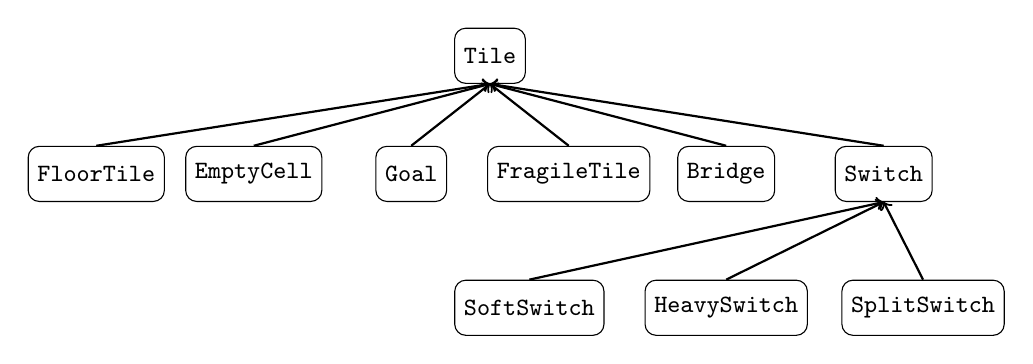
\begin{tikzpicture}[
        box/.style={
            draw, rounded corners,
            minimum height=0.7cm,
            align=center, font=\small
        },
        edge/.style={->, thick}
    ]
        \node[box] (tile) at (0,0) {\texttt{Tile}};

        \node[box] (floor) at (-5,-1.5) {\texttt{FloorTile}};
        \node[box] (empty) at (-3,-1.5) {\texttt{EmptyCell}};
        \node[box] (goal) at (-1,-1.5) {\texttt{Goal}};
        \node[box] (fragile) at (1,-1.5) {\texttt{FragileTile}};
        \node[box] (bridge) at (3,-1.5) {\texttt{Bridge}};
        \node[box] (switch) at (5,-1.5) {\texttt{Switch}};

        \foreach \child in {floor,empty,goal,fragile,bridge,switch}
            \draw[edge] (\child.north) -- (tile.south);

        \node[box] (soft) at (0.5,-3.2) {\texttt{SoftSwitch}};
        \node[box] (heavy) at (3,-3.2) {\texttt{HeavySwitch}};
        \node[box] (split) at (5.5,-3.2) {\texttt{SplitSwitch}};

        \foreach \child in {soft,heavy,split}
            \draw[edge] (\child.north) -- (switch.south);
    \end{tikzpicture}
    \caption{Quan hệ kế thừa giữa các loại ô.
    Mũi tên hướng từ lớp con đến lớp cha.}
    \label{fig:tile_classes}
\end{figure}

\begin{figure}[htbp]
    \centering
    \begin{tikzpicture}[
        box/.style={
            draw, rounded corners,
            minimum width=2.6cm, minimum height=0.8cm,
            align=center, font=\small
        },
        edge/.style={->, thick},
        note/.style={font=\scriptsize, fill=white, inner sep=2pt}
    ]
        \node[box] (solver) at (0,0) {\texttt{BaseSolver}};
        \node[box] (rules) at (4,0) {\texttt{GameRules}};
        \node[box] (board) at (8,0) {\texttt{Board}};
        \node[box] (state) at (8,-1.8) {\texttt{GameState}};
        \node[box] (block) at (4,-1.8) {\texttt{BlockState}};
        \node[box] (tiles) at (8,-3.6) {Các đối tượng \texttt{Tile}};

        \draw[edge] (solver) -- node[note,above]{sử dụng} (rules);
        \draw[edge] (rules) -- node[note,above]{tham chiếu} (board);
        \draw[edge] (board) -- node[note,right]{trạng thái hiện tại} (state);
        \draw[edge] (state) -- node[note,above]{chứa} (block);
        \draw[edge] (board.east) -- ++(1.4,0)
            |- node[note,pos=0.75,right]{quản lý} (tiles.east);
    \end{tikzpicture}
    \caption{Quan hệ sử dụng và chứa giữa các lớp chính,
    không biểu diễn quan hệ kế thừa.}
    \label{fig:backend_relations}
\end{figure}

Các lớp \texttt{BFSSolver}, \texttt{DFSSolver}, \texttt{UCSSolver}
và \texttt{AStarSolver} kế thừa \texttt{BaseSolver}, dùng chung
cách sinh trạng thái và truy vết lời giải.

\subsection{Các hàm cơ sở}
\begin{description}
    \item[\texttt{init\_map(map\_name)}]
    Đọc dữ liệu JSON, tạo các đối tượng trên bàn và khởi tạo
    trạng thái bắt đầu.

    \item[\texttt{Board.initialize\_game\_state()}]
    Khởi tạo trạng thái khối và tập cầu mở theo cấu hình
    \texttt{initial\_open}.

    \item[\texttt{Board.get\_tile(position)}]
    Tra cứu ô tại tọa độ, ưu tiên cầu phủ lên ô nền;
    trả \texttt{None} nếu không có ô.

    \item[\texttt{Board.add\_game\_state(state)}]
    Cập nhật trạng thái hiện tại và đồng bộ thuộc tính khối
    của bàn chơi.

    \item[\texttt{GameRules.is\_valid(state)}]
    Kiểm tra hình dạng khối, cấu hình cầu và khả năng đỡ khối
    tại mọi vị trí đang chiếm giữ.

    \item[\texttt{GameRules.apply\_action(state, action)}]
    Tính trạng thái kế tiếp sau một hành động. Hàm xử lý di chuyển,
    công tắc, cầu và tách/ghép khối; trả \texttt{None} nếu không hợp lệ,
    không sửa bàn chơi hay trạng thái đầu vào.

    \item[\texttt{GameRules.is\_goal(state)}]
    Kiểm tra trạng thái hợp lệ và khối nguyên vẹn đứng thẳng
    trên ô đích.

    \item[\texttt{BaseSolver.successors(state)}]
    Sinh các bộ $(action,next\_state,cost)$ hợp lệ theo thứ tự
    hành động chung, với chi phí mỗi hành động bằng 1.

    \item[\texttt{BaseSolver.reconstruct\_path(goal\_node)}]
    Lần theo \texttt{parent}, thu thập \texttt{action} và đảo
    thứ tự để trả chuỗi hành động từ đầu đến đích.
\end{description}

\subsection{Luồng xử lý hành động}
Với hành động di chuyển, \texttt{apply\_action()} tính tư thế và vị trí mới, kiểm tra khả năng đứng trên các ô, áp dụng công tắc rồi kiểm
tra lại trạng thái sau khi hành động. Nếu khối đang tách, hai khối con sẽ được hợp nhất khi nằm kề nhau. Hành động \texttt{Switch} chỉ đổi
khối đang điều khiển và chỉ hợp lệ khi khối đang được tách.

Giao diện cập nhật bàn chơi bằng trạng thái trả về, các solver dùng trạng thái đó để mở rộng tìm kiếm. Do đó chơi thủ công và phát lại lời
giải đều tuân theo cùng một bộ luật.
